\section{Progressos}

Como foi especificado no documento de especifica��o, n�s seguiremos a arquitetura indicada na figura~\ref{arquitetura:global} abaixo.

\begin{figure}[h]%
\begin{center}
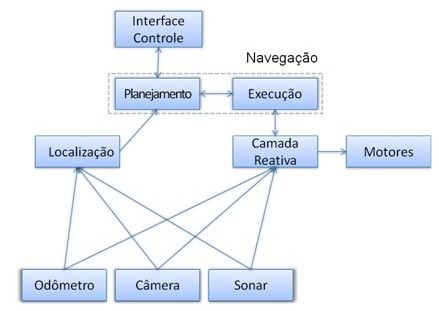
\includegraphics[width=.5\columnwidth]{imagens/arquitetura.jpg}
\caption{Arquitetura do Sistema completo.}%
\label{arquitetura:global}%
\end{center}
\end{figure}

Dentro desta arquitetura, os m�dulos: Od�metro, Sonares e Vis�o s�o considerados prontos. Od�metros e Sonares s�o sensores presentes na plataforma-rob� Pionner P2DX. A Vis�o ser� provida por uma c�mera comercial de baixo custo. Nossos testes est�o sendo realizados com a HS988 da Raysun Shine e com a Microsoft LifeCam VX1000.

Nossos progressos concentraram-se no M�dulo de Localiza��o, cuja arquitetura se baseia no uso do estimador baesiano conhecido por Filtro de Kalman. A arquitetura detalhada do M�dulo de Localiza��o encontra-se na figura~\ref{arquitetura:localizacao} abaixo.

\begin{figure}[h]%
\begin{center}
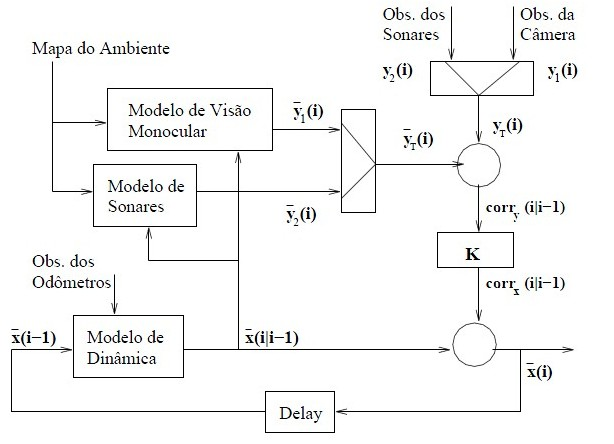
\includegraphics[width=.5\columnwidth]{imagens/arquitetura_localizacao.jpg}
\caption{Arquitetura Detalhada do M�dulo de Localiza��o.\cite{barra}}%
\label{arquitetura:localizacao}%
\end{center}
\end{figure}

O M�dulo de Localiza��o foi o primeiro a ser desenvolvido levando-se em conta sua dificuldade, considerada maior do que dos demais m�dulos. Dessa forma tamb�m seguimos o planejamento realizado anteriormente.

Nas pr�ximas se��es detalharemos os progessos relativos ao M�dulo de Localiza��o e os m�dulos internos, como o Modelo de Din�mica com uso dos od�metros, o Modelo de Observa��o dos Sonares, o Modelo de Observa��o da Cam�ra e o Filtro de Kalman especificamente.